\documentclass[a4paper,12pt]{report}
\usepackage[margin=2.5cm]{geometry}
\usepackage{graphicx}
\usepackage{fancyhdr}
\usepackage{tikz}
\usepackage{lipsum} % For filler text if needed
\usepackage{setspace}
\usepackage{titlesec}
\usepackage{everypage}
\usepackage{caption}
\usepackage{subcaption}

% --- No page numbering for title ---
\pagestyle{fancy}
\fancyhf{}
\setlength{\footskip}{56.99039pt}
\fancyfoot[C]{\thepage}

% --- Bottom-right logo ---
\fancyfoot[R]{
    \raisebox{0.1\textwidth}{
\includegraphics[height=0.25cm]{ressources/for_glory.png}}
}
\begin{document}

% --- Logo Placement with TikZ ---
\begin{tikzpicture}[remember picture, overlay]
    % Top-left: Company Logo
    \node[anchor=north west, xshift=1cm, yshift=-3cm] at (current page.north west) {
        
\includegraphics[width=0.5\textwidth, keepaspectratio]{ressources/ss_horizontal_white_on_black.jpg}
    };
    
    % Top-right: University Logo
    \node[anchor=north east, xshift=-1cm, yshift=-2cm] at (current page.north east) {
        
\includegraphics[width=0.5\textwidth, keepaspectratio]{ressources/logo_upssitech.png}
    };
\end{tikzpicture}

% ------------------------------------------------------------
\vspace*{4cm}

\begin{center}
    \Huge \textbf{Neural-Assisted Feature Matching}\\[1.5cm]
    \LARGE Internship Report\\[1.5cm]
    \large \textbf{Author:} EL OUARRAT Haytam\\
    \textbf{Internship Period:} Mars – August 2025\\
    \textbf{Location:} SteelSeries, Lille, France\\[2cm]
    
    \textbf{Advisors:} Pierre Biret, Damien Granger, Raphaël Greff\\
    \textbf{University Supervisor:} Phillipe Joly \\[2cm]
    
    \large Engineering Degree in Robotics and Interactive Systems \\
    UPSSITECH \\
    University of Toulouse
\end{center}

\vfill

\begin{center}
    \today
\end{center}

% --- Page Break 
\newpage
\tableofcontents
\listoffigures
% ------------------------------------------------------------
\chapter{Acknowledgements}
% ------------------------------------------------------------
\chapter{Introduction}

\section{Host Organism}
\subsection{SteelSeries}
\subsubsection{Company history and Background}
Steel\textbf{Series}, a danish manufacturer of gaming peripherals, was founded in 2001 by Jacob Wolff-Petersen. The company originally launched under the name Soft Trading, and made its mark with innovative gaming mousepads in the early 2000s. In 2007, Soft Trading rebranded to SteelSeries, reflecting its broadened focus beyonf mousepads and into a full range of PC gaming accecories. Key milestones in SteelSeries' evolution include the acquisition of Ideazon in 2008, which brought the Zboard and World of Warcraft gaming keyboard into its portfolio, and further its presence in the North American market.
The company grew rapidly in the 2010s, fueled by its involvement in the esports scene and partnerships with professional gamers. SteelSeries has since expanded its product line to include high-performance gaming mice, keyboards, headsets, and mousepads, becoming a leading brand in the gaming industry.

\subsubsection{Key Products and Technologies}
SteelSeries, renowed for its gaming peripherals and accecories, spanning several product categories. Its product portfolio includes:
\begin{itemize}
    \item \textbf{Gaming Mice:} High-precision mice with customizable buttons and sensors.
    \begin{figure}[h!]
    \centering
    \begin{subfigure}[b]{0.25\textwidth}
        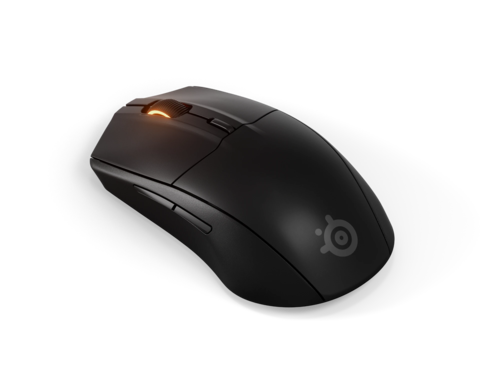
\includegraphics[width=\textwidth]{ressources/mouse_1.png}
        \caption{Rival 3 Wireless Gen 2}
    \end{subfigure}
    \hfill
    \begin{subfigure}[b]{0.25\textwidth}
        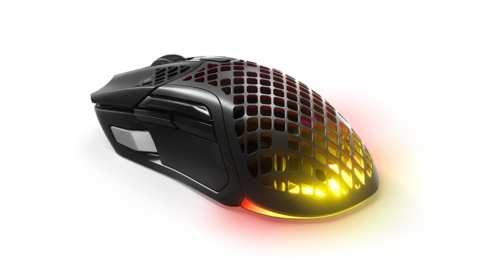
\includegraphics[width=\textwidth]{ressources/mouse_2.png}
        \caption{Aerox 5}
    \end{subfigure}
    \hfill
    \begin{subfigure}[b]{0.25\textwidth}
        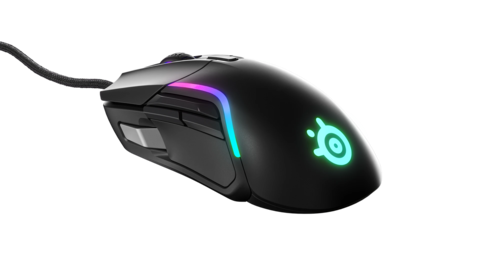
\includegraphics[width=\textwidth]{ressources/mouse_3.png}
        \caption{Rival 5}
    \end{subfigure}
    \caption{SteelSeries Gaming Mice}
    \end{figure}
    \item \textbf{Keyboards:} Mechanical and membrane keyboards designed for gaming performance.
    \begin{figure}[h!]
    \centering
    \begin{subfigure}[b]{0.25\textwidth}
        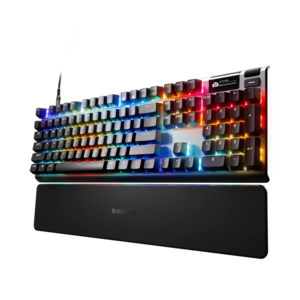
\includegraphics[width=\textwidth]{ressources/kb_1.png}
        \caption{Apex Pro Gen 3}
    \end{subfigure}
    \hfill
    \begin{subfigure}[b]{0.25\textwidth}
        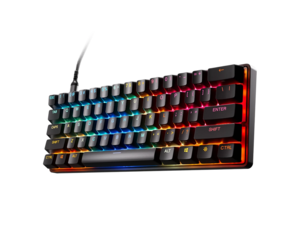
\includegraphics[width=\textwidth]{ressources/kb_2.png}
        \caption{Apex Pro Mini Gen 3}
    \end{subfigure}
    \hfill
    \begin{subfigure}[b]{0.25\textwidth}
        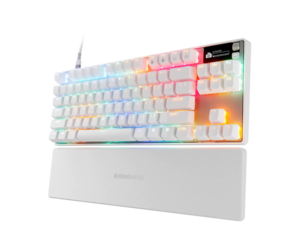
\includegraphics[width=\textwidth]{ressources/kb_3.png}
        \caption{Apex Pro TKL Gen 3}
    \end{subfigure}
    \caption{SteelSeries Gaming Keyboards}
    \end{figure}
    \item \textbf{Headsets:} Wired and wireless headsets with advanced audio features.
    \begin{figure}[h!]
    \centering
    \begin{subfigure}[b]{0.25\textwidth}
        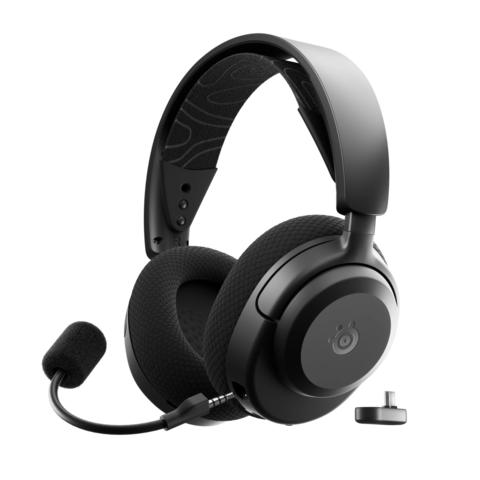
\includegraphics[width=\textwidth]{ressources/hs_2.png}
        \caption{Arctis Nova 3 Wireless}
    \end{subfigure}
    \hfill
    \begin{subfigure}[b]{0.25\textwidth}
        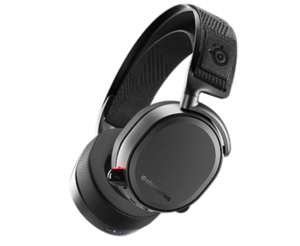
\includegraphics[width=\textwidth]{ressources/hs_3.png}
        \caption{Arctis Pro Wireless}
    \end{subfigure}
    \hfill
    \begin{subfigure}[b]{0.25\textwidth}
        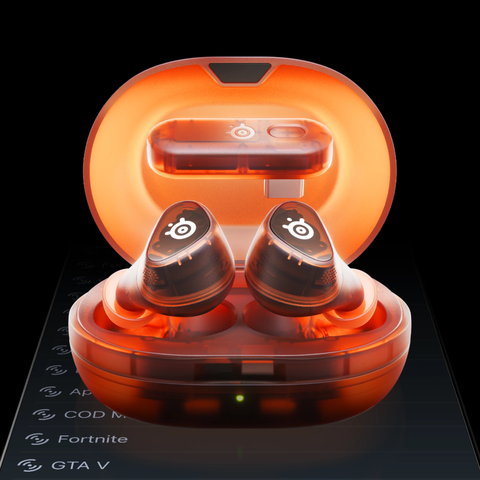
\includegraphics[width=\textwidth]{ressources/hs_1.png}
        \caption{Arctis GameBuds™ Glorange}
    \end{subfigure}
    \caption{SteelSeries Gaming Keyboards}
    \end{figure}
    \item \textbf{Mousepads:} Various sizes and materials optimized for different play styles.
    \item \textbf{Software:}
        \begin{itemize}
        \item \textbf{SteelSeries GG:} the all-in-one software platform that brings together the various tools and services SteelSeries offers to enhance the gaming experience. It serves as the central hub for managing SteelSeries peripherals and includes multiple sub-applications.
        \item \textbf{SteelSeries Engine:} the part of GG that handles the core device configuration. It's used to customize settings for SteelSeries mice, keyboards, headsets, and other gear. Through Engine, users can adjust RGB lighting effects, set up macros, fine-tune mouse sensitivity (DPI).
        \item SteelSeries' advanced audio suite built specifically for gamers who want precise control over their sound experience. It offers a powerful parametric equalizer that lets users independently customize audio for game sounds, voice chat, and microphone input.
        \item \textbf{SteelSeries Moments:} a gameplay capture tool within GG that automatically records key moments during gaming sessions. It can detect in-game events like kills, wins, or goals and save short clips around those events.
        \end{itemize} 
\end{itemize}

\subsection{Mission}
SteelSeries' mission is to create the best gaming gear in the world, empowering gamers to perform at their best, whether it is for professional who seek perfection, or casuals who seek a sense of competition and completion. It's implication over the years in the esports scene has made it a trusted brand among professional gamers, and its commitment to innovation continues to drive the development of new products that enhance the gaming experience. Most notably, SKT Gaming, a professional esports organization, has been using SteelSeries products since 2012, and has won multiple championships in games like CS:GO and League of Legends etc.
\begin{figure}[h!]
    \centering
    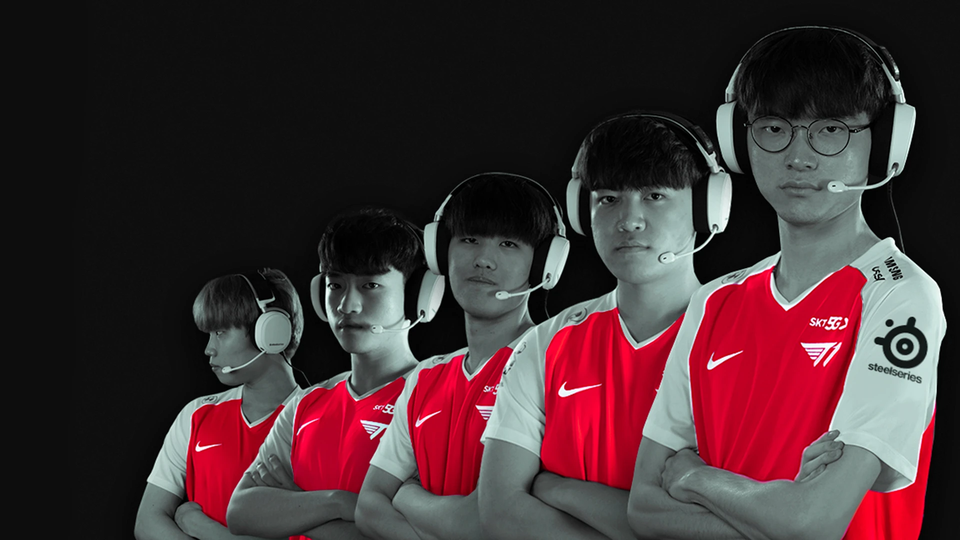
\includegraphics[width=0.7\textwidth]{ressources/sktt1.png}
    \caption{}
    \label{fig:}
\end{figure}
\section{Context \& Motivation}
\subsection{Role of Feature Matching in Computer Vision}
\subsection{Challenges in Gaming Applications}
\subsection{Limitations of Traditional Feature Matching Techniques}

\section{Project Objectives}
\subsection{Reprodusing Feature Matching Techniques with Neural Networks}
\subsection{Improving computational efficiency}
\subsection{Ensure matching accuracy for gaming footage}

\section{Industrial Relevance}
\subsection{Integration with SteelSeries Moments Software}
\subsection{Real-time performance constraints}

% ------------------------------------------------------------
\chapter{Literature Review}
\section{Traditional Feature Matching}
\subsection{Overview of SIFT, ORB, FAST}
\subsection{Comparative Strengths, Weaknesses, and Computational Costs}

\section{Neural Feature Matching}
\subsection{Review of Recent Methods: LoFTR, ALIKE, LightGlue, XFeat}

\section{Knowledge Distillation}
\subsection{Distillation Types: Response-Based, Feature-Based, Relation-Based}
\subsection{Applications in Model Compression and Matching Tasks}

\section{Lightweight Architectures for Edge Deployment}
\subsection{MobileNet, ShuffleNet, XFeat-Style Networks}
\subsection{Trade-Offs Between Efficiency and Accuracy}

\section{Gaps and Opportunities}
\subsection{Where Traditional Methods Fall Short}
\subsection{Where Neural Methods Remain Overkill for Real-Time CPU Usage}
\subsection{Motivation for a Hybrid/Distilled Approach}

% ------------------------------------------------------------
\chapter{Methodology}
\section{Problem Formulation}
\subsection{Define Feature Matching as Correspondence Prediction}
\subsection{Objectives in Terms of Speed, Accuracy, and Robustness}

\section{Baseline Selection}
\subsection{Justification for Using ORB or FAST as Teacher Models}
\subsection{Benchmark Datasets (e.g., HPatches, Gaming Clips)}

\section{Neural Architecture Design}
\subsection{Choice of Lightweight CNN or Transformer Backbone}
\subsection{Feature Extraction vs. Matching Separation}

\section{Distillation Strategy}
\subsection{Design of Teacher-Student Framework}
\subsection{Distillation Losses (e.g., L2 on Descriptors, Cross-Entropy on Match Maps)}

\section{Evaluation Metrics}
\subsection{Matching Precision, Recall, Repeatability}
\subsection{Runtime (FPS), Memory Footprint, CPU Load}

% ------------------------------------------------------------
\chapter{Implementation}
\section{Dataset Preparation}
\subsection{Gaming Video Frame Extraction}
\subsection{Synthetic Transformation Generation for Ground Truth Correspondences}

\section{Training Pipeline}
\subsection{Data Augmentation Strategies}
\subsection{Loss Function Components and Training Schedule}

\section{Model Optimization}
\subsection{Quantization, Pruning, or ONNX Export (if applicable)}
\subsection{Inference Optimization for CPU}

\section{Integration with SteelSeries Pipeline}
\subsection{Data Flow Alignment with Moments Software (if available)}
\subsection{Latency Tracking and Bottleneck Identification}

% ------------------------------------------------------------
\chapter{Results \& Analysis}
\section{Matching Quality}
\subsection{Quantitative Comparison with ORB, SIFT, and XFeat}
\subsection{Visual Results on Gaming Footage}

\section{Computational Efficiency}
\subsection{FPS and Latency Benchmarks}
\subsection{Memory and CPU Usage Profiles}

\section{Ablation Studies}
\subsection{Effect of Different Distillation Losses}
\subsection{Model Depth vs. Performance Trade-Offs}

\section{Real-Time Viability}
\subsection{End-to-End Latency Breakdown}
\subsection{Suitability for Gaming Hardware}

% ------------------------------------------------------------
\chapter{Conclusion and Future Work}
\section{Summary of Contributions}
\section{Limitations}
\subsection{Domain Generalization}
\subsection{Extreme Low-Light or High-Motion Scenes}

\section{Future Work}
\subsection{Self-Distillation or Online Distillation Strategies}
\subsection{Hardware-Specific Optimizations (e.g., ARM CPU Tuning)}
\subsection{Real-Time Deployment on End-User Devices}


% ------------------------------------------------------------
\chapter{References}
% ------------------------------------------------------------
\chapter{Appendices}
\section{Additional Figures}
\section{Code Snippets}
\section{Hyperparameter Tables}
\section{Hardware Specifications}
% ------------------------------------------------------------
\end{document}
